\section{Accesibilidad en la web}

%-----------------------    ---------------------------------

\begin{frame}
\frametitle{¿Por qué accesibilidad?}

\begin{itemize}
   \item El porcentaje de ciudadanos en España con algún tipo de discapacidad se estima en el 9\% (INE 2002), aunque en USA se eleva este número al 20\% (US Census, 1997)
   \item Con el creciente envejecimiento, crecerá en los próximos años
   \item (Si todo va bien) En algún momento, nosotros mismos seremos personas con problemas de accesibilidad
   \item Aún así, la mayoría de los sitios presentan numerosas barreras de accesibilidad
\end{itemize}

\end{frame}


%-----------------------    ---------------------------------

\begin{frame}
\frametitle{Introducción a la accesibilidad}

\begin{enumerate}
   \item Deficiencias visuales
   \item Deficiencias auditivas
   \item Deficiencias motrices
   \item Deficiencias cognitivas y de lenguaje
\end{enumerate}

La discapacidad no es el único tipo de limitación que dificulta la accesibilidad de contenidos. También hay situaciones derivadas del contexto de uso y del dispositivo.

\end{frame}

%-----------------------    ---------------------------------

\begin{frame}
\frametitle{¿Qué podemos hacer?}

\begin{itemize}
  \item Pautas de Accesibilidad al Contenido en la Web 1.0: http://www.discapnet.es/web_accesible/wcag10/WAI-WEBCONTENT-19990505_es.html
\end{itemize}

Entre ellas:

\begin{enumerate}
   \item Validar la sintaxis (Por ejemplo, HTML, XML, etc.).
   \item Validar las hojas de estilo (Por ejemplo, CSS).
\end{enumerate}

Hay numerosas herramientas que ayudan a la validación: \url{http://www.usableyaccesible.com/recurso\_misvalidadores.php}

Algunas requieren revisión manual.

\end{frame}


%-----------------------    ---------------------------------

\begin{frame}
\frametitle{}

\begin{center}
  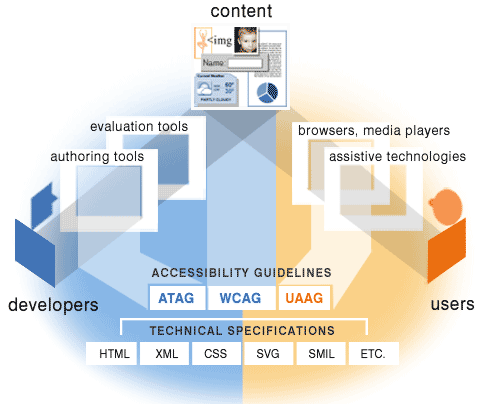
\includegraphics[width=10cm]{figs/accesibilidad.png}
\end{center}


\begin{flushright}
{\tiny
Source: \url{http://www.w3.org/WAI/intro/specs}
}
\end{flushright}

\end{frame}


